A hidden layer in a neural network is one of the layers of neurons between the input layer and the ouput layer. Each layer consists of columns of neurons, and are connected to neurons in adjacent layers. The connections between these neurons are called weights, and are represented by a real number value. These weights are individual, meaning that two neurons in the same layer, recieving the same input, can have different weights associated to it. A neuron in a hidden layer, takes as input, all of the attached neurons multiplied by their weight, summed including a fixed bias and passed through an activation function to a scalar-output. This activation function is in our case a rectified linear unit.\\

\noindent
% Kig lige på Wouters kommentar til den her linje
Presenting this as a function, the sum of the multiplied weights and added bias we define as $y_i$. We then define the connected neurons $x_j$ for $j \in$ \{1,...,N\}, where N is the amount of the connected neurons. We define the associated weights as $w_{ij}$ and added bias as $b_i$. Having the activation function as $\sigma$:

\begin{align}
  y_i &= \sum^N_{j=1} x_jw_{ij} + b_i\\
  a_i &= \sigma(y_i)
\end{align}


\begin{figure}[!ht]
  \centering
  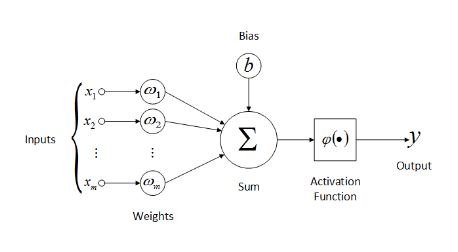
\includegraphics[scale=1.0]{latex/imgs/neuronFunc.png}
  \caption{Diagram representing how a neuron calculates its value}\label{Baseline:before}
\end{figure}

\noindent
When training a neural network, the only parameters that change are the weights. Since the weight from the neuron(1) is multiplied with the weight connecting to neuron(2), the magnitude of this weight defines how much influence neuron(1) has on neuron(2). Thus, the quality of the model depends on how good it is at adjusting the weights, and by that teaching the model to map an input to a correct output.
